
%=========================================================
\section{Módulos del sistema}

%    El sistema se encuentra organizado por módulos con la finalidad de agrupar y administrar de mejor manera los requerimientos funcionales del sistema. Dividir el sistema en módulos permite visualizar e identificar rápidamente aquellos aspectos funcionales que pueden tratarse conjuntamente. \\
%
%    La figura \ref{fig:ModulosPAEAR} muestra los módulos propuestos de manera inicial para el \saear. Cada uno de estos módulos agrupan los casos de uso que poseen funcionalidad similar o que trabajan en conjunto para alcanzar un aspecto funcional del sistema. Cada uno de los módulos que se muestran en la figura se describen a continuación:

    \begin{figure}[h!]
	\begin{center}
	     % \fbox{\includegraphics[width=\textwidth]{images/modulos.jpg}}
%	\caption{Módulos del \saear.}
%	\label{fig:ModulosPAEAR}
	\end{center}
    \end{figure}

    \begin{itemize}
	\item {\bf Proceso de admisión:} Agrupa los casos de uso que tienen que ver con el proceso de admisión para los aspirantes a la Escuela Libre de Derecho. 

	%\item {\bf Proceso de inscripción} Agrupa los casos de uso que permiten a los aspirante aceptados, así como a los alumnos de semestres arriba poder inscribirse a un nuevo ciclo escolar.
	
	\item {\bf Proceso de gestión académica:} Agrupa los casos de uso que tienen que ver con el proceso de gestión académica de la Escuela Libre de Derecho. 
	
	\item {\bf Proceso de estructuración académica:} Agrupa los casos de uso que tienen que ver con el proceso de estructuración académica de la Escuela Libre de Derecho. 
    \end{itemize}

%=========================================================
\section{Actores del sistema}\label{sec:Comportamiento:ActoresSistema}

Los actores son los perfiles asociados a las diversas áreas y/u organizaciones que intervienen en el proceso. Se han identificado los actores de acuerdo a las actividades y responsabilidades dentro del \sae, los cuales se muestran en la figura \ref{fig:perfilesPAEAR} y se describen a continuación.

%    \begin{figure}[h!]
%      \begin{center}
%	  \includegraphics[width=0.6\textwidth]{images/actores/Actores.png}
%      \caption{Perfiles identificados.}
%      \label{fig:perfilesPAEAR}
%      \end{center}
%    \end{figure}

%ASPIRANTE
    \cdtLabel{Actor:Aspirante}{}
    \begin{actor}{Aspirante}{-----}

	\item[Área:] Persona externa a la Escuela Libre de Derecho.

	\item[Responsabilidades:] \hspace{1pt}
	
		\begin{itemize}
		    \item Crear una cuenta de usuario para el registro de su información necesario para comenzar el proceso de ingreso a la Escuela Libre de Derecho. 
		    \item Registrar su información personal para comenzar con el proceso de admisión
		    \item Realizar el pago de derechos a exámenes
		    \item Realizar su registro para el EXANI-II
		 \end{itemize}
	\item[Perfil:] \hspace{1pt}
		\begin{itemize}
		    \item Persona interesada en ingresar como alumno a la Escuela Libre de Derecho, debe estar cursando el último año de educación media superior o ser egresado de nivel medio superior o equivalente.
	    \end{itemize}
	\item[Cantidad:] No se define.
\end{actor}


%COORDINACION DE CONTROL ESCOLAR 
\cdtLabel{Actor:CCE}{}
\begin{actor}{Coordinación de Control Escolar}{-----}
	
	\item[Área:] Secretaría de Administración - Control Escolar.
	
	\item[Responsabilidades:] \hspace{1pt}
	    \begin{itemize}
	    	\item Gestionar las etapas del calendario escolar de la Escuela Libre de Derecho.
	        \item Definir los Requisitos y Criterios para la convocatoria de ingreso a la Escuela Libre de Derecho.
	        \item Realizar el registro de un aspirante en caso de que este justifique que no puede hacerlo.
	        \item Gestionar el proceso para la aplicación del EXANNI-II de CENEVAL.
	        \item Gestionar el proceso para la aplicación de las entrevistas para los aspirantes a la Escuela Libre de Derecho.
	    \end{itemize}
	\item[Perfil:] \hspace{1pt}
	\begin{itemize}
		\item Lic. en Control Escolar
	\end{itemize}
	\item[Cantidad:] Uno por la Escuela Libre de Derecho.
\end{actor}


%RESPONSABLE DE CONTROL ESCOLAR
\cdtLabel{Actor:RCE}{}
\begin{actor}{Responsable de Control Escolar}{-----}
	
	\item[Área:] Secretaría de Administración - Control Escolar.
	
	\item[Responsabilidades:] \hspace{1pt}
%	\begin{itemize}
%		\item Gestionar las etapas del calendario escolar de la Escuela Libre de Derecho.
%		\item Definir los Requisitos y Criterios para la convocatoria de ingreso a la Escuela Libre de Derecho.
%		\item Realizar el registro de un aspirante en caso de que este justifique que no puede hacerlo.
%		\item Gestionar el proceso para la aplicación del EXANNI-II de CENEVAL.
%		\item Gestionar el proceso para la aplicación de las entrevistas para los aspirantes a la Escuela Libre de Derecho.
%	\end{itemize}
	\item[Perfil:] \hspace{1pt}
	\begin{itemize}
		\item Lic. en Control Escolar
	\end{itemize}
	\item[Cantidad:] %Uno por la Escuela Libre de Derecho.
\end{actor}


%ASISTENTE DE LA Secretaría DE ADMINISTRACIÓN
%\cdtLabel{Actor:ASA}{}
%\begin{actor}{Asistente de la Secretaría de Administración}{-----}
%	
%	\item[Área:] Escuela Libre de Derecho - Secretaría de Administración.
%	
%	\item[Responsabilidades:] \hspace{1pt}
%	\begin{itemize}
%		\item Registrar en sistema las fechas para generar el calendario escolar de la Escuela Libre de Derecho.
%	\end{itemize}
%	\item[Perfil:] \hspace{1pt}
%	\begin{itemize}
%		\item Conocer el área de Secretaría de Administración
%	\end{itemize}
%	\item[Cantidad:] Uno por la Escuela Libre de Derecho.
%\end{actor}

%Secretaría DE ADMINISTRACIÓN
\cdtLabel{Actor:SA}{}
\begin{actor}{Secretaría de Administración}{-----}
	
	\item[Área:] Escuela Libre de Derecho - Secretaría de Administración.
	
	\item[Responsabilidades:] \hspace{1pt}
	
	\begin{itemize}
		\item Revisar el calendario escolar registrado en el sistema.
		\item Llevar a la Junta Directiva de la Escuela Libre de Derecho la propuesta de calendario escolar para su aprobación.
	\end{itemize}
	\item[Perfil:] \hspace{1pt}
	\begin{itemize}
		\item Conocer el área de Secretaría de Administración
	\end{itemize}
	\item[Cantidad:] Uno por la Escuela Libre de Derecho:
\end{actor}


%ENTREVISTADOR
\cdtLabel{Actor:Entrevistador}{}
\begin{actor}{Entrevistador}{-----}
	
	\item[Área:] Escuela Libre de Derecho o externos
	
	\item[Responsabilidades:] \hspace{1pt}
	
	\begin{itemize}
		\item Entrevistar a los aspirantes a la Escuela Libre de Derecho que le sean asignados.
	\end{itemize}
	\item[Perfil:] \hspace{1pt}
	\begin{itemize}
		\item Personal de la Escuela Libre de Derecho o Egresado.
	\end{itemize}
	\item[Cantidad:] Los requeridos para la cantidad de entrevistas necesarias.
\end{actor}


%COORDINADOR DE PSICOLOGOS
\cdtLabel{Actor:CP}{}
\begin{actor}{Coordinador de Psicólogos}{-----}
	
	\item[Área:] Externo
	
	\item[Responsabilidades:] \hspace{1pt}
	
	\begin{itemize}
		\item Registrar resultados del examen electrónico.
		\item Validar las evaluaciones de los psicólogos.
	\end{itemize}
	\item[Perfil:] \hspace{1pt}
	\begin{itemize}
		\item Licenciado en psicología.
	\end{itemize}
	\item[Cantidad:] Uno.
\end{actor}


%PSICOLOGO
\cdtLabel{Actor:Psicologo}{}
\begin{actor}{Psicólogo}{-----}
	
	\item[Área:] Externos
	
	\item[Responsabilidades:] \hspace{1pt}
	
	\begin{itemize}
		\item Entrevistar a los aspirantes a la Escuela Libre de Derecho que le sean asignados.
		\item Evaluar los resultados de las pruebas psicométricas.
	\end{itemize}
	\item[Perfil:] \hspace{1pt}
	\begin{itemize}
		\item Licenciado en psicología.
	\end{itemize}
	\item[Cantidad:] Los requeridos para la cantidad de entrevistas y evaluaciones necesarias.
\end{actor}


%PROFESOR
\cdtLabel{Actor:Profesor}{}
\begin{actor}{Profesor}{-----}
	
	\item[Área:] Escuela Libre de Derecho
	
	\item[Responsabilidades:] \hspace{1pt}
	
	\begin{itemize}
		\item Impartir clases a los alumnos de las materias que le fueron asignadas.
	\end{itemize}
	\item[Perfil:] \hspace{1pt}
	\begin{itemize}
		\item Profesor de la Escuela Libre de Derecho o Egresado.
	\end{itemize}
	\item[Cantidad:] Los requeridos para impartir las materias.
\end{actor}

%=========================================================

%Alumno
\cdtLabel{Actor:Alumno}{}
\begin{actor}{Alumno}{-----}
	
	\item[Área:] Escuela Libre de Derecho
	
	\item[Responsabilidades:] \hspace{1pt}
	
	\begin{itemize}
		\item Realizar pago de inscripción.
		\item Realizar pago de colegiaturas.
		\item Realizar reinscripción a grados superiores.
	\end{itemize}
	\item[Perfil:] \hspace{1pt}
	\begin{itemize}
		\item Alumno de la Escuela Libre de Derecho.
	\end{itemize}
	\item[Cantidad:] No se define.
\end{actor}


%====================================================================================
\section{Casos de Uso del módulo de Consulta de Profesores}

La figura \ref{fig:casosUso:generacionCalendario} muestra los casos de uso que integran la funcionalidad del módulo de Generación de calendario escolar, que se refieren al registro, modificación y visualización de los ciclos escolares así como la información de las etapas y actividades asociadas a cada ciclo escolar.

\begin{figure}[h!]
	\begin{center}
		\fbox{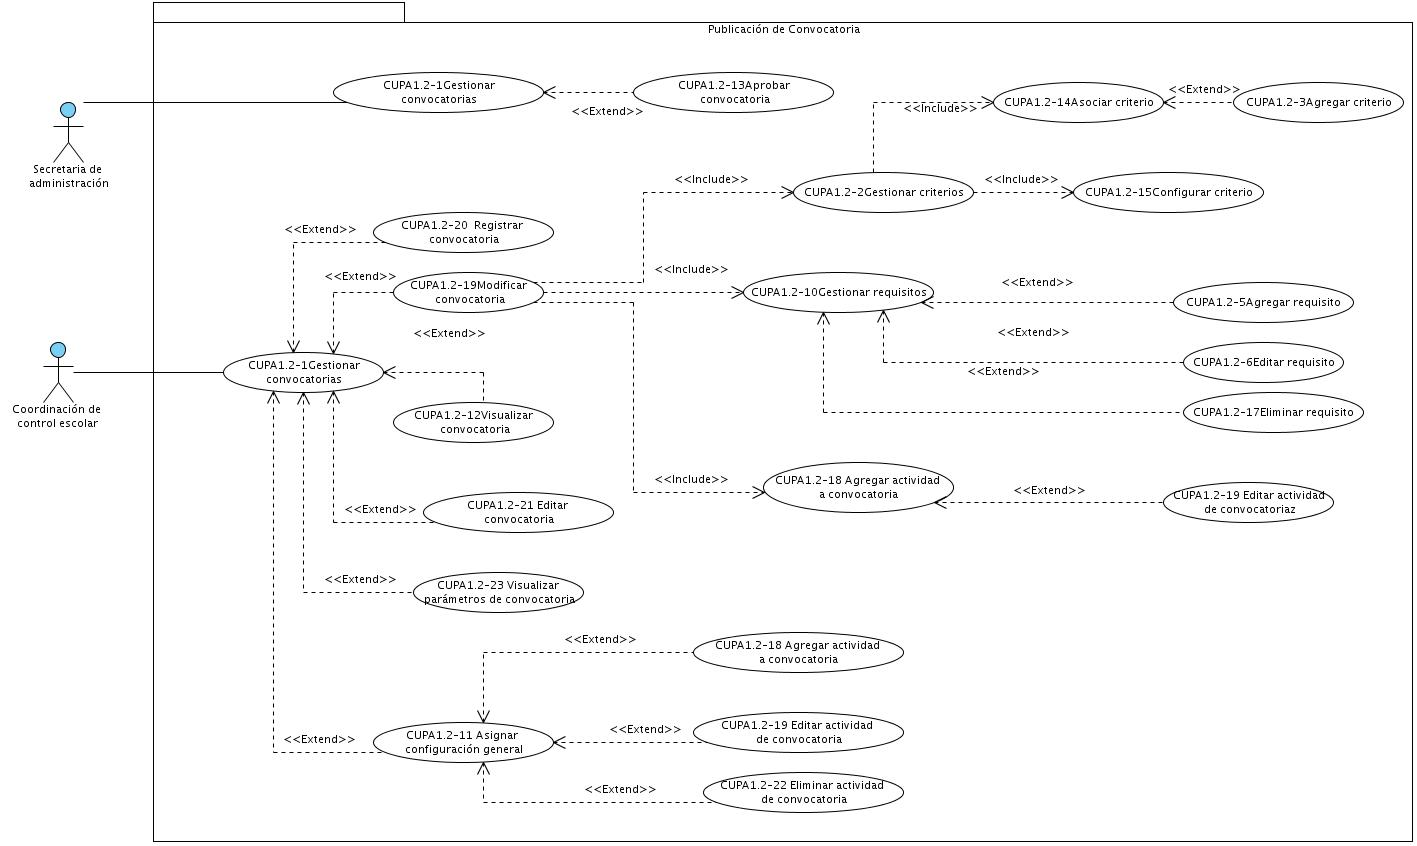
\includegraphics[width=.9\textwidth]{ModeloComportamiento/modulo-consultaDeProfesores/images/DCU_consulta_de_profesores}}
		\caption{Diagrama de casos de uso para el módulo de Generación de Calendario Escolar. \label{fig:casosUso:generacionCalendario}}
	\end{center}
\end{figure}

%====================================================================================
\section{Casos de Uso del módulo de Horarios}

La figura \ref{fig:casosUso:generacionConvocatoria} muestra los casos de uso que integran la funcionalidad del módulo de Generación de Convocatoria de Ingreso, que se refieren al registro, modificación y visualización de las convocatorias de ingreso que se pueden generar en los ciclos.

\begin{figure}[h!]
	\begin{center}
		\fbox{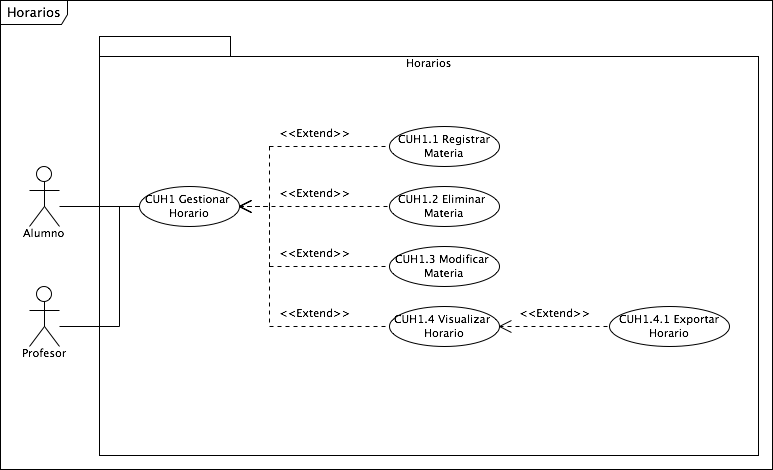
\includegraphics[width=.9\textwidth]{ModeloComportamiento/modulo-horarios/images/DCU_horarios}}
		\caption{Diagrama de casos de uso para el módulo de Generación de Convocatoria de Ingreso. \label{fig:casosUso:generacionConvocatoria}}
	\end{center}
\end{figure}
